\documentclass[a4paper, 12pt]{article}
\usepackage[T2A]{fontenc}
\usepackage[utf8]{inputenc}
\usepackage[english,russian]{babel}
\usepackage{amsmath, amsfonts, amssymb, amsthm, mathtools, misccorr, indentfirst, multirow, multicol}
\usepackage{wrapfig}
\usepackage{graphicx}
\usepackage{subfig}
\usepackage{adjustbox}
\usepackage{pgfplots}

\usepackage{geometry}
\geometry{top=20mm}
\geometry{bottom=20mm}
\geometry{left=20mm}
\geometry{right=20mm}
\newcommand{\angstrom}{\textup{\AA}}

\title{Лабораторная работа № 4.3.1\\Изучение дифракции света}
\author{Нехаев Александр 654 гр.}
\date{\today}
\begin{document}
	\maketitle
	\newpage
	\tableofcontents
	\newpage
	\section{Введение}
	\paragraph{Цель работы} Изучить дифракцию Френеля и Фраунговера, в том числе на двойной щели. Исследовать  влияние дифракции на разрешающую способность данной оптической системы.
	\paragraph{Оборудование} Оптическая скамья, ртутная лампа, монохроматор, щели с регулируемой шириной, рамка с вертикальной нитью, двойная щель, микроскоп на поперечных салазках с микрометрическим винтом, зрительная труба.
	\subsection{Теоретическая основа}
	\subsubsection{Дифракция Френеля}
	Щель $S_2$ освещается параллельным пучком монохроматического света с помощью коллиматора, образованного объективом $O_1$ и щелью $S_1$, находящейся в его фокусе. На щель $S_1$ сфокусировано изображение спектральной линии, выделенной из спектра ртутной лампы $\text{Л}$ при помощи простого монохроматора $C$, в котором используется призма прямого зрения\par
	\begin{wrapfigure}{1}{7cm}
		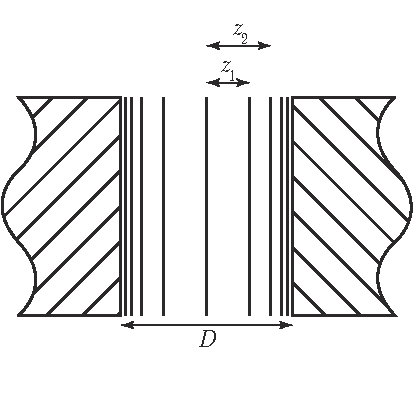
\includegraphics[scale=0.9]{Fig1.pdf}
		\caption{Зоны Френеля в области щели}
		\label{pic:1}
	\end{wrapfigure}

	Распределение интенсивности света в плоскости наблюдения $\Pi$ проще всего рассчитывать с помощью зон Френеля (для щели их иногда называют зонами Шустера). При освещении щели $S_2$ параллельным пучком лучей (плоская волна) зоны Френеля представляют собой полоски, параллельные краям щели (рис. \ref{pic:1}). Результирующая амплитуда в точке наблюдения определяется суперпозицией колебаний от тех зон Френеля, которые не перекрыты створками щели.Графическое определение результирующей амплитуды производится с помощью векторной диаграммы — спирали Корню. Суммарная ширина $m$ зон Френеля $z_m$ определяется соотношением:
	\begin{equation*}
		z_m=\sqrt{am\lambda}
	\end{equation*}
	где $a$ — расстояние от щели до плоскости наблюдения, $\lambda$ — длина волны.\par
	Вид наблюдаемой дифракционной картины определяется числом Френеля, а квадрат:
	\begin{equation}
		\Phi^2=\frac{D}{\sqrt{a\lambda}}
	\end{equation}
	— это соотношение ширины щели $D$ к размеру первой зоны Френеля, т.е. число зон Френеля, которое укладывается на ширине щели. Обратную величину называют \textit{волновым параметром}.\par
	Дифракционная картина отсутствует, когда плоскость наблюдения $\Pi$ совпадает с плоскостью щели: при $\Phi\rightarrow\infty$ мы имеем дело с геометрической оптикой. При небольшом удалении от щели, когда число зон Френеля $\Phi\gg 1$ (на щели укладывается огромное число зон), распределение интенсивности света за щелью также можно получить с помощью законов геометрической оптики (приближенно). Дифракционная картина в этом случае наблюдается только в узкой области на границе света и тени у краев экрана.
	\subsubsection{Дифракция Фраунгофера на щели}
	\begin{wrapfigure}{1}{7cm}
		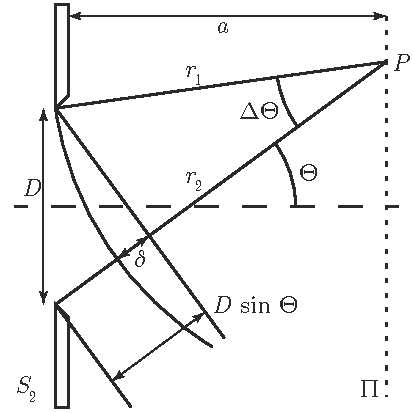
\includegraphics[scale=0.9]{Fig2.pdf}
		\caption{К фазовым соотношениям при дифракции Фраунгоферв}
		\label{pic:2}
	\end{wrapfigure}

	Картина дифракции резко упрощается, когда ширина щели становится значительно меньше ширины первой зоны Френеля, т.е. если
	\begin{equation}
		D\ll\sqrt{a\lambda}\quad\text{или}\quad\Phi\ll 1
		\label{condition:2}
	\end{equation}
	Это условие всегда выполняется при достаточно большом расстоянии $a$ от щели до плоскости наблюдения. Дифракционную картину, наблюдаемую в этом случае, принято называть дифракцией Фраунгофера. Исследование такой дифракционной картины заметно облегчается, потому что упрощаются фазовые соотношения. Это поясняет рис. \ref{pic:2}. При выполнении условия (\ref{condition:2}) разность хода между крайними лучами, приходящими от щели в точку наблюдения $P$, с хорошим приближением можно вычислять по формуле
	\begin{equation}
		\Delta=D\sin\Theta.
		\label{eq:3}
	\end{equation}
	Здесь предполагается, что дифракционный угол $\Theta$ достаточно мал, так что $\sin\Theta\approx\Theta$. Формула (\ref{eq:3}) справедлива при условии $\delta\ll\lambda/2$. Можно показать, что это условие эквивалентно условию (\ref{condition:2}).\par
	\begin{wrapfigure}{1}{7cm}
		\includegraphics[scale=0.25]{Fig31.png}
		\caption{Распределение интенсивности при дифракции Фраунгофера на щели}
		\caption{pic:3}
	\end{wrapfigure}
	Дифракцию Френеля и Фраунгофера можно наблюдать на одной и той же установке (рис. 5). Однако при обычных размерах установки дифракция Фраунгофера возникает только при очень узких щелях. Например, при $a\approx20-40$ см. и $\lambda\approx5\cdot10^{-5}$ см. получаем $D\ll0.3$ мм. Поскольку работать с такими тонкими щелями неудобно, для наблюдения дифракции Фраунгофера к схеме, изображенной на рис. 1 добавляется объектив $O_2$ (рис. 6).\par
	Дифракционная картина наблюдается здесь в фокальной плоскости объектива $O_2$. Каждому значению угла $\Theta$ соответствует в этой плоскости точка, отстоящая от оптической оси на расстоянии:
	\begin{equation}
		X=f_2\tan\Theta
		\label{eq:4}
	\end{equation}
	Поскольку объектив не вносит дополнительной разности хода между интерферирующими лучами (таутохронизм), в его фокальной плоскости наблюдается неискаженная дифракционная картина Фраунгофера. Эта картина соответствует бесконечно удалённой плоскости наблюдения. Распределение интенсивности в дифракционной картине Фраунгофера представлено на рис. 3.\par
	Поскольку при $\Theta=0$ разность хода между любой парой лучей равна нулю, в центре поля зрения наблюдается дифракционный максимум (светлая полоса). Первый минимум (первая темная полоса) соответствует, очевидно, такому значению дифракционного угла $\Theta_1$, при котором в точке наблюдения разность хода пробегает все возможные значения от нуля до $2\pi$. Рассуждая аналогичным образом, можно определить угловую координату $\Theta_m$ любой тёмной полосы. Для малых углов
	\begin{equation}
		m\lambda=D\Theta_m
		\label{eq:5}
	\end{equation}
	Расстояние $X_m$ тёмной полосы от оптической оси объектива $O_2$ пропорционально фокусному расстоянию $f_2$. Из (\ref{eq:4}) и (\ref{eq:5}) следует:
	\begin{equation}
		X_m=f_2m\frac{\lambda}{D}.
		\label{eq:6}
	\end{equation}
	Из (\ref{eq:6}) видно, что при малых углах минимумы эквидистантны, а расстояния $\Delta X$ между минимумами обратно пропорциональны ширине $D$ щели $S_2$.
	\subsubsection{Дифракция Фраунгофера на двух щелях}
	Для наблюдения дифракции Фраунгофера на двух щелях (рис. 4) следует заменить щель $S_2$ экраном $\text{Э}$ с двумя щелями (рис. 6). При этом для оценки влияния ширины входной щели на четкость дифракционной картины вместо входной щели $S_1$ следует поставить щель с микрометрическим винтом. Два дифракционных изображения входной щели, одно из которых образовано лучами, прошедшими через левую, а другое — через правую щели, накладываются друг на друга.\par
	Если входная щель достаточно узка, то дифракционная картина в плоскости $\Pi$ (рис. 6) подобна той, что получается при дифракции на одной щели (рис. 4), однако теперь вся картина испещерена рядом дополнительных узких полос. Наличие этих полос объясняется суперпозицией световых волн, приходящих в плоскость наблюдения через разные щели экрана $\text{Э}$. В центре главного дифракционного максимума (рис. 6) располагается светлая полоса, так как при $\theta=0$ разность хода между этими волнами равна нулю (все лучи, приходящие в фокус объектива $O_2$, синфазны). Светлая интерференционная полоса наблюдается и во всех тех случаях, когда указанная разность хода равна целому числу длин волн. Таким образом, угловая координата $\theta_m$ интерференционная полоса наблюдается и во всех тех случаях, когда указанная разность хода равна целому числу длин волн. Таким образом, угловая координата $\theta_m$ интерференционного максимума $m$-го порядка определяется соотношением:
	\begin{equation}
		d\theta_m=m\lambda
	\end{equation}
	где $d$ — расстояние между щелями.\par
	Линейное расстояние $\delta x$ между соседними интерференционными полосами в плоскости $\Pi$ равно поэтому
	\begin{equation}
		\delta x=f_2\frac{x}{d}
	\end{equation}
	На рис. 6 показано распределение интенсивности в фокальной плоскости объектива $O_2$. Штриховой линией (в увеличенном масштабе) изображено распределение интенсивности при дифракции света на одиночной щели.\par
	Нетрудно оценить число $n$ интерференционных полос, укладывающихся в области центрального дифракционного максимума. Согласно (\ref{eq:6}) полная ширина главного максимума $\frac{2 f_2\lambda}{D}$, где $D$ — ширина щели, отсюда
	\begin{equation}
		n=\frac{2\lambda f_2}{D}\frac{1}{\delta x},\quad \text{т.е. }n=\frac{2d}{D}
	\end{equation}
	При дифракции света на двух щелях чёткая система интерференционных полос наблюдается только при достаточно узкой ширине входной щели $S$. При увеличении её ширины интерференционная картина периодически пропадает и появляется вновь, но полосы при этом оказываются сильно размытыми и видны плохо. Это явление объясняется наложением интерференционных картин от разных элементов широкой щели $S$. Первое размытие интерференционных полос возникает при условии
	\begin{equation}
		\frac{b}{f_1}=\frac{\lambda}{d}
	\end{equation}
	Здесь $b$ — ширина входной щели $S$ и, следовательно, $\frac{b}{f_1}$ — её угловая ширина. Таким образом, по размытию интерференционной картины можно оценить размер источника. Этот метод используется в звёздном интерферометре при измерении угловых размеров звёзд.\par
	\subsubsection{Влияние дифракции на разрешающую способность оптического инструмента}
	Установка, представленная на рис. 4, позволяет исследовать влияние дифракции на разрешающую способность оптических инструментов.\par
	Как уже было выяснено, линзы $O_1$ и $O_2$ в отсутствие щели $S_2$ создают в плоскости $\Pi$ изображение щели $S_1$, и это изображение рассматривается в микроскоп $M$. Таким образом, нашу установку можно рассматривать как оптический инструмент, предназначенный для получения изображения предмета. При этом коллиматор (щель $S_1$ и объектив $O_1$) является модель далёкого предмета, а объектив $O_2$ и микроскоп $M$ составляют зрительную трубу, наведённую на этот предмет.\par
	Если перед объективом $O_2$ зрительной трубы расположить щель $S_2$, то изображение объекта будет искажено дифракцией на щели $S_2$. Чем меньше ширина $D_0$ этой щели, тем сильнее искажение. Качественной характеристики этих искажений может служить минимальное угловое расстояние $\varphi_{\min}$ между которыми равно $d$ (рис. 7). Тогда на щель $S_2$ будут падать два параллельных пучка света, составляющих между собой угол $\varphi$, равный (для малых углов)
	\begin{equation}
		\varphi=\frac{d}{f_1}.
	\end{equation}
	Параллельные лучи 1 и 2, проходящие через центры линз, определяют положения изображений двойной щели. Согласно законам геометрической оптики расстояние $l$ между изображениями щелей в плоскост $\Pi$ равно
	\begin{equation}
		l=\varphi f_2, \quad \text{т.е. }l=d\frac{f_2}{f_1}
	\end{equation}
	а ширина $\Delta\varphi$ каждого изображения определяется дифракцией света на щели $S_2$. Когда полуширина дифракционного изображения превышает расстояние между изображениями, то ввиду дифракционной картины трудно определить, представляет собой источник двойную щель или одиночную. Предельные условия, при которых ещё можно различить, имеем мы дело с одной или с двумя щелями, для разных наблюдателей различны.\par
	\begin{wrapfigure}{1}{6cm}
		\includegraphics[scale=0.2]{Fig4.png}
		\caption{Критерий разрешения по Рэлею}
		\label{pic:5}
	\end{wrapfigure}
	Для того чтобы исключить связанный с этим произвол, пользуются обычно критерием Рэлея, который приблизительно соответствует возможностям визуального наблюдения: изображения считаются различимыми, когда максимум одного дифракционного пятна совпадает с минимумом другого, а в условиях нашей задачи — когда угловая полуширина дифракционного изображения $\frac{\lambda}{D_0}$ совпадает с угловым расстоянием $\varphi = \frac{l}{f_2}$ между изображениями отдельных щелей (рис. 4):
	\begin{equation*}
		\frac{\lambda}{D_0}=\frac{l}{f_2}\quad\text{и}\quad\frac{l}{f_2}=\frac{d}{f_1}
	\end{equation*}
	\section{Практическая часть}
	\subsection{Дифракция Френеля}
	Собираем схему с рис. \ref{exp_scheme_1} и и на первую щель фокусируем зеленую часть спектра, затем отмеряем положение микрометрического винта на щели и настраиваем зрительную трубу на бесконечность, получая четкую картину, убираем трубу и ставим на её место микроскоп. Также добиваемся четкости картины, фокусируя микроскоп на щель 2.
	\begin{figure}[h]
		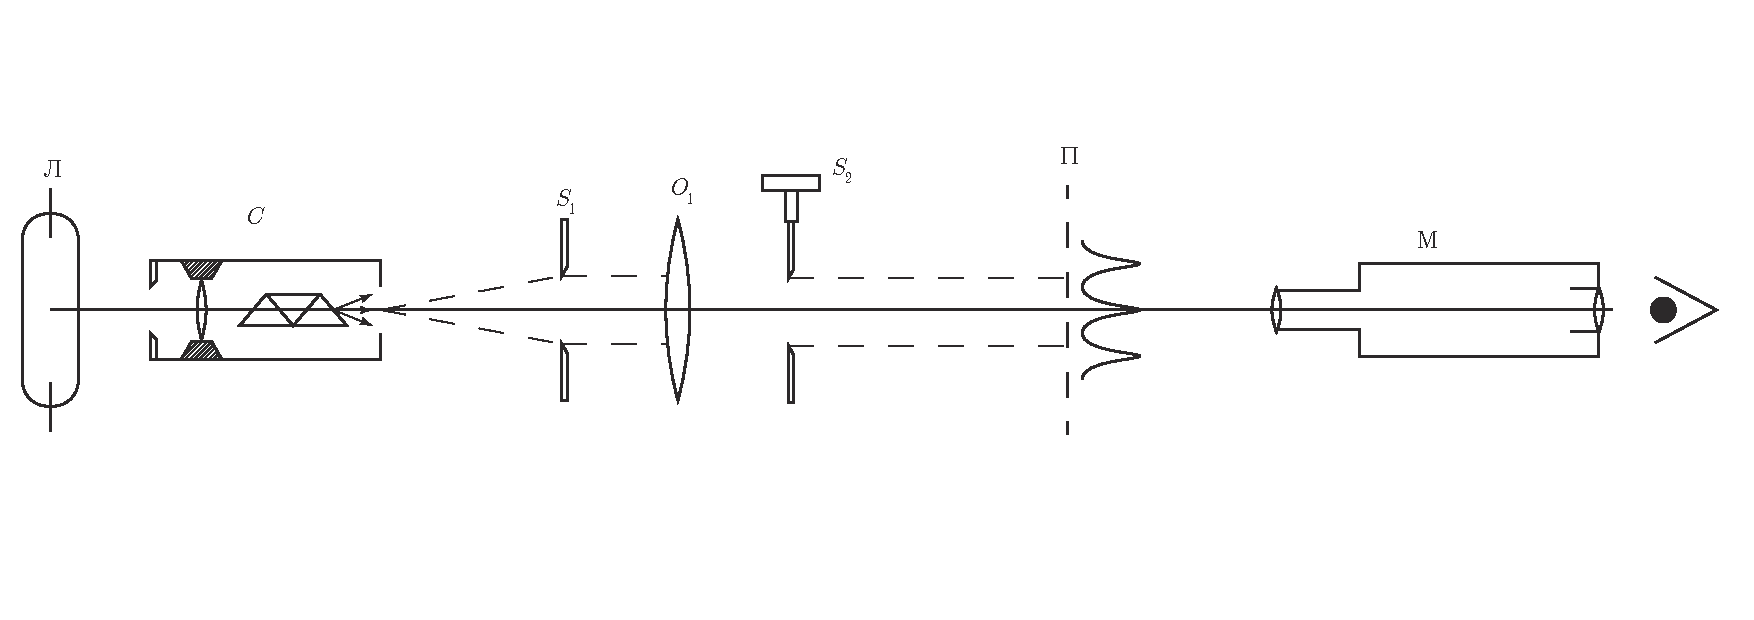
\includegraphics[scale=0.55]{scheme1.pdf}
		\caption{Схема установки для наблюдения дифракции Френеля}
		\label{exp_scheme_1}
	\end{figure}
	\begin{equation*}
		F_1=15.5\text{ см}, \quad F_2=16\text{ см}.
	\end{equation*}
	Нуль микрометрического винта на 20 делениях(каждое деление 0.001 мм).
	Открываем щель 2 на $D=250\text{ дел}=0.25 \text{ мм}$, измерение проводится на микрометрическом винте щели.\\
	Аналогичное измерение проводим с помощью внутренней шкалы микроскопа (цена деления 0.02 мм) $D=11 \text{ дел}=0,22 \text{ мм}$.\\
	При сравнении $b$ практически совпадают.\\
	Cнимаем зависимость координаты микроскопа от числа n наблюдаемых тёмных полос.\\
	$a$-расстояние между микроскопом и щелью.\\
	Cравниваем размер зон Френеля с измеренной шириной $D$ щели $S_2$. Для этого связываем число тёмных полос $n$ в поле зрения с числом зон Френеля $m$ на полуширине щели, рассчитаем величину $2z_m$ по формуле: $z_m=\sqrt{am\lambda}$ при $\lambda=5461 \angstrom = 546.1$ нм. Полученные значения $2z_m$ занесем в таблицу \ref{tab:1}:\\
	\begin{table}[h]
		\centering
		\begin{tabular}{|c|c|c|}
			\hline
			$m$ & $a$, мм & $2z_m$, мкм\\
			\hline
			1 & 63 & 370.968\\
			2 & 60 & 511.984\\
			3 & 58 & 616.511\\
			4 & 57 & 705.722\\
			5 & 56 & 782.069\\
			\hline
		\end{tabular}
		\caption{Зависимость $2z_m$ от $m$.}
		\label{tab:1}
	\end{table}
	По значениям таблицы построим график (рис. \ref{graph1:1})
	\begin{figure}
		\begin{tikzpicture}
			\begin{axis}[
				title={$2z_m=f(m)$},
				xlabel={$m$},
				ylabel={$2z_m$, мкм},
				xmin=1,
				xmax=5,
				ymin=370,
				ymax=785,
				ymajorgrids=true,
   				xmajorgrids=true,
	 			grid style=dashed,
	 			width=\textwidth,
			]
			\addplot+[
	 				color=black,
					mark=square,
					only marks,
					error bars/.cd,
					y dir=both, y explicit,
					x dir=both, x explicit
	 		]
	 		coordinates{
	 			(1, 370.968)+-(0, 29.4)
	 			(2, 511.984)+-(0, 42.6)
	 			(3, 616.511)+-(0, 53.1)
	 			(4, 705.722)+-(0, 61.9)
	 			(5, 782.069)+-(0, 69.8)
	 		};
	 		\addplot[
	 			domain=1:6,
	 			samples=100,
	 			color=black
	 		]
	 		{101.594*x+292.669};
			\end{axis}
		\end{tikzpicture}
		\caption{Зависимость ширины зоны Френеля от её номера.}
		\label{graph1:1}
	\end{figure}
	\subsection{Дифракция Фраунгофера на щели}
	\begin{figure}[h]
		\centering
		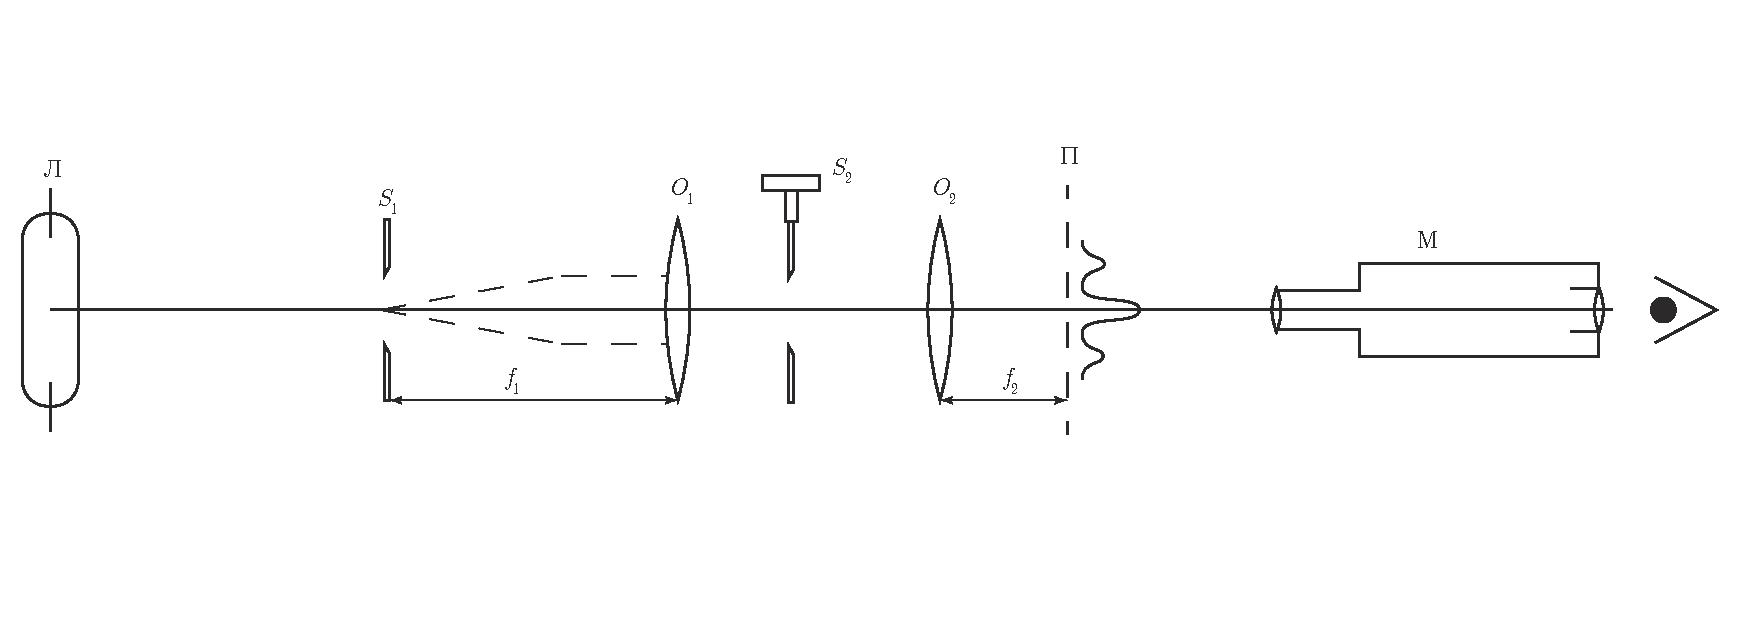
\includegraphics[scale=0.55]{scheme2.pdf}
		\caption{Схема установки для изучения дифракции Фраунгофера на щели}
		\label{exp_scheme_2}
	\end{figure}
	Измеряем с помощью винта поперечного перемещения микроскопа координаты $X_m$ нескольких дифракционных минимумов (от $-m$ до $+m$). Определим ширину $D$ щели $S_2$ и запишем фокусное расстояние линзы $O_2$.
	\begin{equation*}
		F_2=16\text{ см}, \quad D=0.38\text{ мм}
	\end{equation*}
	$b$ — координаты минимумов.\par
	Меряем координаты минимумом с учетом того, что ноль находится в центре 0 минимума, самой яркой центральной полосы.\par
	\begin{table}[h]
		\centering
		\begin{tabular}{|c|c|c|}
			\hline
			$m$ & $b$, дел & $b$, мм\\
			\hline
			3 & 43 & 0.86\\
			2 & 30 & 0.6\\
			1 & 16 & 0.32\\
			-1 & -17 & -0.34\\
			-2 & -31 & -0.62\\
			-3 & -44 & -0.88\\
			\hline
		\end{tabular}
		\caption{Зависимость $b(m)$.}
	\end{table}
	По полученной таблице построим график $b=f(m)$ (рис. \ref{graph})
	\begin{figure}[h]
		\centering
		\begin{tikzpicture}
			\begin{axis}[
				title={$b=f(m)$},
				xlabel={$m$},
				ylabel={$b$, мм},
				xmin=-4,
				xmax=4,
				ymin=-1,
				ymax=1,
				ymajorgrids=true,
   				xmajorgrids=true,
	 			grid style=dashed,
	 			width=\textwidth,
			]
			\addplot+[
	 				color=black,
					mark=square,
					only marks,
					error bars/.cd,
					y dir=both, y explicit,
					x dir=both, x explicit
	 		]
	 		coordinates{
	 			(-3, -0.88)+-(0, 0.07)
	 			(-2, -0.62)+-(0, 0.07)
	 			(-1, -0.34)+-(0, 0.07)
	 			(1, 0.32)+-(0, 0.07)
	 			(2, 0.6)+-(0, 0.07)
	 			(3, 0.86)+-(0, 0.07)
	 		};
	 		\addplot[
	 			domain=-4:4,
	 			samples=100,
	 			color=black
	 		]
	 		{0.2971*x-0.01};
			\end{axis}
		\end{tikzpicture}
		\caption{График зависимости $b(m)$}
		\label{graph}
	\end{figure}
	Среднее значение расстояния между соседними минимумами $\Delta b = 15$ мм.\\
	Рассчитываем размер щели по формуле: $X_m=f_2m\frac{\lambda}{D}$.\\
	$X_m=b\Rightarrow D=0.35$ мм.
	Наблюдения: Чем меньше щель, тем шире интервалы между соседними минимумами.
	\subsection{Дифракция Фраунгофера на двух щелях}
	Определим линейное расстояние $\delta x$ между крайними соседними интерференционными полосами.\par
	$\delta x = 37$ дел. $ = 0.74$ мм.\par
	$x=40$ дел. $=0.80$ мм. — ширина центрального максимума.\par
	Рассчитаем $d$ — расстояние между щелями: $\delta x=f_2\frac{x}{d}$ отсюда $d=\frac{f_2x}{\delta x}$, $d=172.97$ мм.\par
	Рассчитаем число полос внутри главного максимума по формуле: $n=\frac{2d}{D}$.\par
	Теоретическое число полос $n=9.8=10$ полос.\par
	Практическое число полос $n=9$.\par
	Теоретическая ширина щели: $b=\frac{\lambda f_1}{d}=0.41$ мм.\par
	Практическая ширина щели: $b_0=0.39$ мм.
	\section{Вывод}
	В проделанной работы была исследована дифракция Френеля, Фраунгофера на одной и двух щелях. Дифракцию Фраунгофера на двух щелях не удалось изучить подробно по причине слишком узких и размытых дифракционных полос.
\end{document}
